\documentclass[11pt]{article}
\usepackage[margin=1in]{geometry}
\usepackage{graphicx}
\usepackage{hyperref}
\usepackage{xcolor}
\usepackage{booktabs}
\usepackage{enumitem}
\usepackage{float}
\usepackage{caption}
\usepackage{amsmath}
\usepackage{listings}
\usepackage{tikz}
\usetikzlibrary{positioning, arrows.meta, fit, backgrounds, calc}

\definecolor{codebg}{rgb}{0.95,0.95,0.95}
\definecolor{codegreen}{rgb}{0,0.5,0}
\definecolor{codegray}{rgb}{0.5,0.5,0.5}
\definecolor{codepurple}{rgb}{0.5,0,0.33}

\lstset{
    backgroundcolor=\color{codebg},
    basicstyle=\ttfamily\footnotesize,
    breaklines=true,
    frame=single,
    numbers=left,
    numberstyle=\tiny\color{codegray},
    keywordstyle=\color{codepurple},
    commentstyle=\color{codegreen},
    stringstyle=\color{blue},
    showstringspaces=false,
    tabsize=2
}

\title{Coverage-Guided Fuzzing of NVIDIA Dynamo:\\Finding Bugs in a Production LLM Inference Framework}
\author{Shounak Ray, Arpit Ranasaria}
\date{March 2026}

\begin{document}
\maketitle

\begin{abstract}
We applied coverage-guided fuzzing to NVIDIA Dynamo, an open-source LLM inference framework with over 6,000 GitHub stars. Across 46 fuzz targets spanning 5 Rust crates, we found 16 previously unknown bugs: a critical integer overflow in a network-facing codec, 6 high-severity bugs (panics, deadlocks, logic errors, and data corruption), and 9 medium-severity issues. We submitted a fix for the critical overflow that was approved by NVIDIA's team, and a second bug was independently fixed upstream during our campaign. The most useful thing we learned: the choice of oracle strategy matters more than the fuzzer itself. Crash-only testing missed entire categories of bugs that differential and semantic oracles caught in seconds.
\end{abstract}

\enlargethispage{2\baselineskip}
\tableofcontents
\newpage

%% ============================================================
\section{System Description}
%% ============================================================

We used \textbf{coverage-guided fuzzing} to find bugs in NVIDIA Dynamo~\cite{dynamo}, a production LLM inference framework written primarily in Rust. The fuzzer generates random inputs, feeds them to a program, and uses code coverage feedback to steer generation toward unexplored paths. When the program crashes or violates an expected property, the fuzzer saves the triggering input. We use \texttt{libFuzzer}~\cite{libfuzzer} via the \texttt{cargo-fuzz}~\cite{cargofuzz} Rust wrapper.

Dynamo handles KV-cache-aware request routing, tool-call parsing for function calling, network communication between distributed workers, and token block management. The codebase is roughly 150,000 lines of Rust, actively developed by 200+ contributors, and deployed in production at NVIDIA for LLM serving. Figure~\ref{fig:architecture} shows the architecture and request flow.

\begin{figure}[H]
\centering
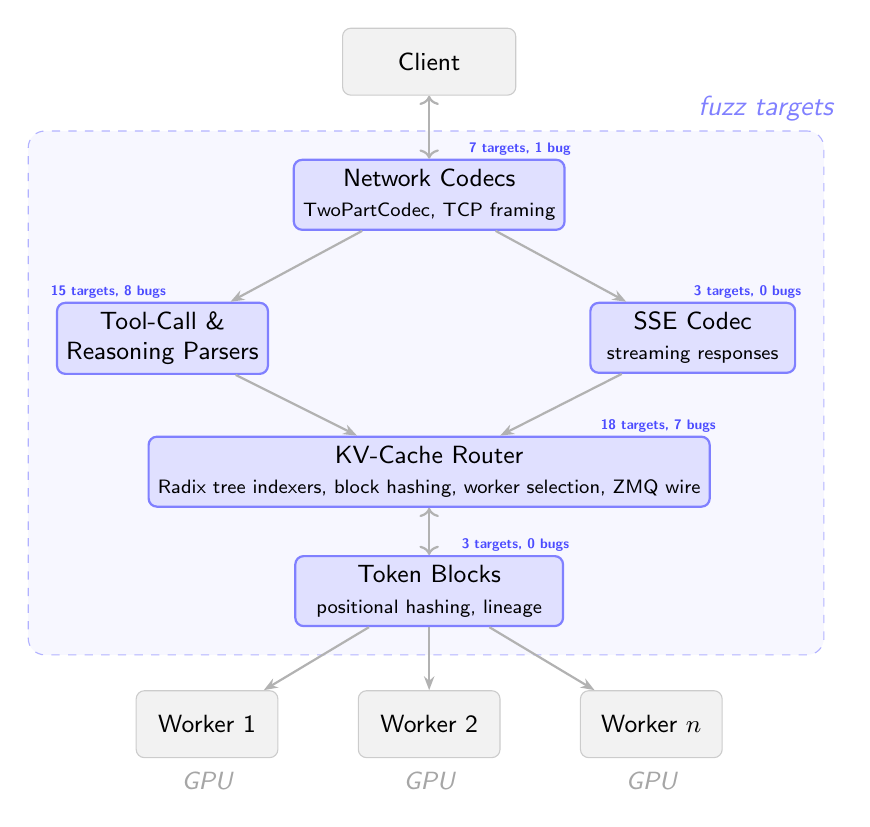
\begin{tikzpicture}[
    node distance=0.6cm and 1.2cm,
    box/.style={draw, rounded corners=3pt, minimum height=0.85cm, minimum width=2.6cm,
                align=center, font=\small\sffamily},
    fuzzed/.style={box, fill=blue!12, draw=blue!50, line width=0.8pt},
    unfuzzed/.style={box, fill=gray!10, draw=gray!40},
    lbl/.style={font=\scriptsize\sffamily\itshape, text=gray!70},
    arr/.style={-{Stealth[length=5pt]}, thick, gray!60},
    darr/.style={arr, <->},
    stat/.style={font=\sffamily\bfseries\tiny, text=blue!70},
]

% --- Client ---
\node[unfuzzed, minimum width=2.2cm] (client) {Client};

% --- Runtime layer ---
\node[fuzzed, below=0.8cm of client, minimum width=3.2cm] (codec)
    {Network Codecs\\\scriptsize TwoPartCodec, TCP framing};

% --- Middle processing layer ---
\node[fuzzed, below left=0.9cm and 0.3cm of codec] (parsers)
    {Tool-Call \&\\Reasoning Parsers};
\node[fuzzed, below right=0.9cm and 0.3cm of codec] (sse)
    {SSE Codec\\\scriptsize streaming responses};

% --- KV-Router layer ---
\node[fuzzed, below=2.6cm of codec, minimum width=5.8cm] (kvrouter)
    {KV-Cache Router\\\scriptsize Radix tree indexers, block hashing, worker selection, ZMQ wire};

% --- Token layer ---
\node[fuzzed, below=0.6cm of kvrouter, minimum width=3.4cm] (tokens)
    {Token Blocks\\\scriptsize positional hashing, lineage};

% --- Workers ---
\node[unfuzzed, below left=0.8cm and 0.2cm of tokens, minimum width=1.8cm] (w1) {Worker 1};
\node[unfuzzed, below=0.8cm of tokens, minimum width=1.8cm] (w2) {Worker 2};
\node[unfuzzed, below right=0.8cm and 0.2cm of tokens, minimum width=1.8cm] (w3) {Worker $n$};

% --- GPU labels ---
\node[lbl, below=0.05cm of w1] {\small GPU};
\node[lbl, below=0.05cm of w2] {\small GPU};
\node[lbl, below=0.05cm of w3] {\small GPU};

% --- Arrows ---
\draw[darr] (client) -- (codec);
\draw[arr] (codec) -- (parsers);
\draw[arr] (codec) -- (sse);
\draw[arr] (parsers) -- (kvrouter);
\draw[arr] (sse) -- (kvrouter);
\draw[darr] (kvrouter) -- (tokens);
\draw[arr] (tokens) -- (w1);
\draw[arr] (tokens) -- (w2);
\draw[arr] (tokens) -- (w3);

% --- Stats (targets / bugs) ---
\node[stat, inner sep=0pt, anchor=south east] at ([yshift=1pt, xshift=2pt]codec.north east)
    {7 targets, 1 bug};
\node[stat, inner sep=0pt, anchor=south west] at ([yshift=1pt, xshift=-2pt]parsers.north west)
    {15 targets, 8 bugs};
\node[stat, inner sep=0pt, anchor=south east] at ([yshift=1pt, xshift=2pt]sse.north east)
    {3 targets, 0 bugs};
\node[stat, inner sep=0pt, anchor=south east] at ([yshift=1pt, xshift=2pt]kvrouter.north east)
    {18 targets, 7 bugs};
\node[stat, inner sep=0pt, anchor=south east] at ([yshift=1pt, xshift=2pt]tokens.north east)
    {3 targets, 0 bugs};

% --- Fuzz target annotation ---
\begin{scope}[on background layer]
    \node[draw=blue!30, dashed, rounded corners=6pt, fill=blue!3,
          fit=(codec)(parsers)(sse)(kvrouter)(tokens),
          inner sep=10pt, label={[lbl, text=blue!50]above right:{\normalsize fuzz targets}}] {};
\end{scope}

\end{tikzpicture}
\caption{Dynamo architecture with fuzzed components highlighted. Shaded boxes are the 5 crates we targeted. We focused most of our effort on the Parsers and KV-Cache Router, but fuzzed targets lightly across all highlighted components. Arrows show request/response flow from client through network codecs, parsing and routing layers, down to GPU workers.}
\label{fig:architecture}
\end{figure}

We targeted 5 core library crates that process untrusted or semi-structured input:

\begin{itemize}[nosep]
    \item \textbf{lib/parsers}: Tool-call parsers for 14+ LLM output formats (XML, JSON, DSML, Pythonic, GLM-4.7, KimiK2, etc.) plus reasoning parsers (DeepSeek, Granite, MiniMax, etc.)
    \item \textbf{lib/kv-router}: KV-cache routing logic including radix tree indexers, block hash computation, worker selection, and ZMQ wire protocol handling
    \item \textbf{lib/runtime}: Network codecs (TwoPartCodec, TCP framing), event plane serialization, and slug generation
    \item \textbf{lib/tokens}: Token block sequences, positional hashing, and lineage hash computation
    \item \textbf{lib/llm}: Server-Sent Events (SSE) codec for streaming LLM responses
\end{itemize}

Across these crates, we targeted five classes of bugs: panics and crashes (division by zero, out-of-bounds access, integer overflow, UTF-8 boundary violations), logic errors (incorrect indexer scores, wrong function name extraction, stale cached state), data corruption and loss (silent parameter drops, string value corruption, streaming content loss), concurrency bugs (deadlocks in concurrent data structures), and serialization bugs (encode-decode asymmetries in network protocols).

We chose these crates through a manual code audit. Before writing any fuzz targets, we searched the codebase for dangerous patterns: unchecked indexing, unchecked arithmetic, unsafe string slicing at byte offsets, panicking \texttt{unwrap()} calls on external input, and global mutable state. The audit turned up several likely bugs early on, which confirmed these crates were worth targeting and guided our prioritization. We started with the parsers crate (pure-function string processing, easiest to harness) and progressed to the kv-router crate (stateful harnesses, more complex input generation).

%% ============================================================
\section{Technical Overview}
%% ============================================================

This section covers the oracle strategies that define what counts as a bug, how our approach changed based on what we saw working (and not working), and the input generation techniques we used to reach deeper code paths.

\subsection{Oracle Strategies}

Each of the 5 target crates has its own \texttt{fuzz/} directory containing fuzz target source files, seed corpora, dictionaries, and shared helper libraries. The basic structure of a fuzz target is shown below:

\begin{lstlisting}[caption={Basic crash oracle fuzz target}]
#![no_main]
use libfuzzer_sys::fuzz_target;

fuzz_target!(|data: &[u8]| {
    if let Ok(s) = std::str::from_utf8(data) {
        let _ = some_parser::parse(s);
    }
});
\end{lstlisting}

Most of our targets go beyond simple crash oracles. In practice, what you define as a bug matters at least as much as which fuzzer you run. We implemented six oracle strategies, each defining ``incorrect behavior'' differently. Most targets combine multiple strategies (e.g., a differential target also acts as a crash oracle), so the counts below reflect all targets using each strategy, with overlap.

\textbf{Crash oracles} (30+ targets) are the simplest: feed arbitrary bytes to a function, see if it crashes. One useful property of our setup: \texttt{cargo-fuzz} compiles targets in debug mode, where Rust enables arithmetic overflow checks, bounds checks, and debug assertions that are stripped in release builds. Integer overflow that silently wraps in production triggers a panic under fuzzing instead. So crash oracles actually catch bugs that would show up as silent data corruption in deployed code. Nearly all of our 46 targets include implicit crash detection, and about 30 use it as their primary oracle. They work best for network codecs and hash functions, where inputs are untrusted and the code was not written to handle arbitrary bytes.

\textbf{Differential oracles} (4 targets) compare two implementations that should produce identical results. We compare streaming vs. one-shot parsing of the same input (any mismatch indicates a bug in one code path), and we run the same sequence of operations against three independent indexer implementations (RadixTree, ConcurrentRadixTree, PositionalIndexer) and assert their scores match. This ``triple differential'' approach found bugs that no crash oracle could detect.

\textbf{Roundtrip oracles} (7 targets) serialize data, deserialize it, re-serialize, and assert the bytes are identical. We applied this to the ZMQ wire protocol, the TwoPartCodec network framing, the event plane serialization, and positional hash encodings.

\textbf{Consistency oracles} (10+ targets) define semantic properties that must hold for any valid input: any function name a parser extracts must appear as a substring of the original input (no fabrication), reasoning text must grow monotonically across streaming chunks, radix tree query scores must be bounded by the length of the stored sequence, and hash computations must be deterministic. In the ablation study (Section~5), targets where consistency checking is the primary strategy are labeled ``consistency'' to distinguish them from crash-only targets.

\textbf{Semantic oracles} (1 target) embed known-valid tool calls (with known function names and argument values) into fuzz-controlled surrounding text, then verify that the parser extracts them correctly. This catches bugs where a parser extracts wrong data rather than crashing.

\textbf{Stateful/concurrency oracles} (5+ targets) generate sequences of operations (store, remove, clear, query) applied to data structures, checking invariants after each step. One target also spawns concurrent threads to test for deadlocks.

\subsection{Design Evolution}

We did not design this strategy upfront. It evolved as we watched what worked and what didn't.

We started with crash-only harnesses. For the codec and kv-router crates, this worked immediately: the TwoPartCodec crash target found a critical integer overflow within seconds. But the parser crash targets found \textbf{zero bugs despite millions of executions}. The parsers are designed to handle arbitrary model output gracefully: malformed input produces an empty result, never a panic.

That null result forced us to rethink. We switched to differential and semantic oracles that define what ``correct'' means rather than waiting for the program to crash. The differential harness quickly found parser bugs that crash-only testing had missed entirely. Same code, same fuzzer, different oracle, different results. The quantitative comparison is in Section~5.

The same pivot worked for kv-router. We built a stateful harness that generates sequences of store, remove, clear, and query operations against the radix tree, checking invariants after each step. This found an aliasing panic with a 10-byte input. We then built a differential harness comparing the single-threaded \texttt{RadixTree} against the \texttt{ConcurrentRadixTree} and \texttt{PositionalIndexer}, which uncovered a deadlock in the concurrent implementation (Bug~2) and a score underreporting bug (Bug~15) that NVIDIA's team later fixed independently.

We then ran LLVM coverage reports over the accumulated corpus to find blind spots. Several parsers had 0\% coverage from generic targets because they required format-specific input structure. We built targeted harnesses for those (e.g., \texttt{fuzz\_glm47\_utf8} for multibyte handling, \texttt{fuzz\_xml\_deep} with structured inputs for nested argument extraction), which turned up additional bugs.

Finally, we had to deal with known bugs dominating fuzzing results. One crash was so trivially triggerable that it caused the fuzzer to crash and restart on nearly every input, blocking exploration of deeper code paths. The standard workaround of catching panics in the harness was not available: AddressSanitizer, which \texttt{cargo-fuzz} enables by default, intercepts panic unwinding and aborts the process. We solved this by detecting and skipping inputs that trigger known bugs at the harness level, checking preconditions before passing input to the function under test. With this filtering, the same targets found additional bugs that had been unreachable before.

\subsection{Input Generation and Infrastructure}

Many targets use the \texttt{Arbitrary} trait~\cite{arbitrary} to generate structured fuzz inputs rather than raw bytes. This way, mutations are more likely to produce valid-looking inputs that reach deeper code paths instead of being rejected by format validation. Section~5 quantifies the coverage advantage.

Each fuzz crate includes seed corpora (hand-crafted valid inputs for each format), token dictionaries (format-specific keywords), and shared helper libraries for common operations like chunking strings along UTF-8 boundaries and constructing valid event structures. The full source for all targets and infrastructure is available in our repository.\footnote{\url{https://github.com/ShounakRay/fuzzy-dynamo}}

%% ============================================================
\section{System Setup Steps}
%% ============================================================

All code, fuzz targets, seed corpora, dictionaries, crash artifacts, and scripts are in the \texttt{fuzzy-dynamo} repository, a fork of \texttt{ai-dynamo/dynamo}. The following steps reproduce our setup:

\begin{enumerate}[nosep]
    \item \textbf{Clone the repository:} \texttt{git clone https://github.com/ShounakRay/fuzzy-dynamo.git \&\& cd fuzzy-dynamo}
    \item \textbf{Install system libraries.} On Ubuntu: \texttt{sudo apt install build-essential libhwloc-dev libudev-dev pkg-config libclang-dev protobuf-compiler python3-dev cmake}. On macOS: \texttt{brew install cmake protobuf}.
    \item \textbf{Install Rust:} \texttt{curl -{}-proto '=https' -{}-tlsv1.2 -sSf https://sh.rustup.rs | sh} and then install the nightly toolchain and cargo-fuzz: \texttt{rustup install nightly \&\& cargo +nightly install cargo-fuzz}.
    \item \textbf{Run all fuzz targets:} \texttt{./fuzzing/run.sh} (defaults to 60s per target). Filter by crate (\texttt{-{}-crate parsers}) or target (\texttt{-{}-target fuzz\_differential}). Adjust timeout with \texttt{FUZZ\_TIMEOUT=300}.
    \item \textbf{Run individual targets directly:} \texttt{cd lib/parsers \&\& cargo +nightly fuzz run fuzz\_tool\_call\_parsers -{}-  -max\_total\_time=60}.
    \item \textbf{Generate LLVM coverage reports:} \texttt{./fuzzing/coverage.sh}.
\end{enumerate}

Full build-from-source instructions (including Python bindings and optional GPU components) are in the repository README.

%% ============================================================
\section{Evaluation Methodology}
%% ============================================================

We evaluate along three dimensions: what bugs were found and how, how much code was exercised, and how oracle strategy choice affects outcomes.

\textbf{Metrics.} For each fuzz target we record coverage edges (unique control-flow transitions exercised), coverage features (a finer-grained metric including edge hit-count buckets), corpus size (unique coverage-contributing inputs), executions per second, total executions, new crashes, and peak memory usage.

\textbf{Bug detection.} Bugs are detected through four mechanisms: natural panics (Rust panics on out-of-bounds access, integer overflow, unwrap failures), assertion oracles (explicit assertions in fuzz targets that flag undesirable non-crashing behavior), overflow checks (optionally enabled to catch integer overflows that silently wrap in release mode), and AddressSanitizer (integrated by default for memory safety issues).

\textbf{Oracle validation.} We validate each oracle type by confirming it can detect known bugs. For each oracle strategy, we constructed or identified a known-buggy input and verified that the harness flags it within seconds. For example, we verify that the crash oracle rediscovers known panics, that the differential oracle catches a known streaming mismatch, and that the roundtrip oracle catches the TwoPartCodec integer overflow using a saved crash artifact.

\textbf{Ablation study.} To quantify the impact of oracle strategy choice, we designed two types of comparisons. First, our \texttt{ablation.sh} script runs all 46 targets at three time budgets (10s, 30s, 60s), recording coverage, corpus size, throughput, crashes, and time-to-first-crash for each. This provides aggregate data across oracle types and time budgets, though different oracle types are applied to different code, which limits direct comparison.

Second, to isolate individual variables, we built \textbf{controlled pair experiments}: pairs of fuzz targets that test the same underlying code with exactly one variable changed. For input structure, we created \texttt{Arbitrary}-derived structured variants alongside existing raw-byte targets for the same functions (e.g., \texttt{fuzz\_zmq\_wire\_roundtrip} vs. \texttt{fuzz\_zmq\_wire\_roundtrip\_structured}). For known-bug filtering, we created unfiltered variants that omit the guards skipping known crashes (e.g., \texttt{fuzz\_request\_extra\_info} vs. \texttt{fuzz\_request\_extra\_info\_unfiltered}). Each pair was run with an empty corpus at 10s, 30s, and 60s to ensure fair comparison.

\textbf{Production application.} The system under test is NVIDIA Dynamo itself: actively maintained by 200+ contributors, with an existing test suite, deployed in production for LLM serving. All bugs we report were found in this production codebase, not in hand-crafted test programs. Section~6 evaluates the real-world impact.

%% ============================================================
\section{Basic Evaluation}
%% ============================================================

This section reports quantitative results: the bugs found, coverage achieved, and ablation studies comparing oracle strategies, time budgets, and input generation methods.

\subsection{Bug Discovery Results}

Table~\ref{tab:crashes} summarizes all 16 bugs. Each was found by the fuzzer through crash artifacts or oracle violations. The code audit described in Section~1 guided which components we targeted and how we designed the harnesses.

\begin{table}[H]
\centering
\caption{Summary of all bugs discovered}
\label{tab:crashes}
\footnotesize
\begin{tabular}{@{}clllll@{}}
\toprule
\# & Component & Bug Type & Severity & Discovery & Status \\
\midrule
1  & kv-router & \texttt{chunks\_exact(0)} panic & Medium & Crash oracle & Open \\
2  & kv-router & RwLock deadlock & High & Stateful oracle & Open \\
3  & parsers   & UTF-8 boundary panic & High & Crash oracle & Open \\
4  & kv-router & Jump optimization skip & High & Differential oracle & Open \\
5  & kv-router & ZMQ wire OOB panic & High & Crash oracle & Open \\
6  & parsers   & Regex prefix absorption & High & Semantic oracle & Open \\
7  & parsers   & Silent parameter drop & Medium & Crash oracle & Open \\
8  & parsers   & Streaming content loss & Medium & Differential oracle & Open \\
9  & parsers   & OnceLock stale cache & Medium & Crash oracle & Open \\
10 & parsers   & Trailing newline mismatch & Medium & Differential oracle & Open \\
11 & kv-router & Division by zero & Medium & Crash oracle & Open \\
12 & kv-router & Division by zero & Medium & Crash oracle & Open \\
13 & parsers   & \texttt{strip\_quotes} panic & Medium & Crash oracle & Open \\
14 & parsers   & \texttt{try\_literal\_eval} corruption & Medium & Crash oracle & Open \\
15 & kv-router & Score underreporting & High & Differential oracle & Fixed \\
16 & runtime   & Integer overflow & Critical & Crash oracle & Fixed \\
\bottomrule
\end{tabular}
\end{table}

\subsection{Oracle Strategy Effectiveness}

Different oracle strategies found different classes of bugs (Table~\ref{tab:oracle_effectiveness}). Crash oracles found 10 bugs (panics, overflows, out-of-bounds access, data corruption), differential oracles found 4 (streaming/one-shot mismatches, score underreporting, content loss), the semantic oracle found 1 (regex prefix absorption), and the stateful oracle found 1 (deadlock). Crash-only testing was completely blind to logic errors like score underreporting and streaming mismatches. Without the non-crash oracle types, we would have missed 6 of the 16 bugs.

\begin{table}[H]
\centering
\caption{Bugs found per oracle strategy}
\label{tab:oracle_effectiveness}
\begin{tabular}{@{}lcp{7cm}@{}}
\toprule
Oracle Strategy & Bugs Found & Examples \\
\midrule
Crash-only & 10 & Division by zero, OOB access, integer overflow, UTF-8 panic, data corruption \\
Differential & 4 & Streaming/one-shot mismatch, score underreporting, content loss \\
Semantic & 1 & Regex prefix absorption in function name extraction \\
Stateful & 1 & Deadlock on duplicate block hashes \\
\bottomrule
\end{tabular}
\end{table}

\subsection{Coverage Baseline}

Coverage and throughput vary by orders of magnitude across targets (Table~\ref{tab:coverage_by_crate}). This mostly reflects differences in code complexity, not fuzzing quality. Throughput alone is misleading: the fastest target (684K exec/s) covers only 90 edges, while the slowest (285 exec/s) covers 6,951. Because of this variance, the remaining subsections use controlled comparisons to isolate the variables that actually matter.

\begin{table}[H]
\centering
\caption{Coverage by crate at 60 seconds (targets with $>$0 coverage)}
\label{tab:coverage_by_crate}
\footnotesize
\begin{tabular}{@{}llrrrrr@{}}
\toprule
Crate & Representative Target & Oracle & Cov Edges & Features & Corpus & Exec/s \\
\midrule
parsers   & fuzz\_parser\_stress     & consistency  & 7,864  & 30,580 & 1,723 & 3,188 \\
parsers   & fuzz\_differential       & differential & 6,951  & ---    & 308   & 285 \\
parsers   & fuzz\_deepseek\_variants & crash        & 5,582  & 15,526 & 1,842 & 7,142 \\
parsers   & fuzz\_glm47\_utf8        & crash        & 3,843  & 13,686 & 197   & $<$1 \\
\addlinespace
kv-router & fuzz\_zmq\_wire\_decode  & crash        & 3,481  & 4,827  & 1,493 & 12,637 \\
kv-router & fuzz\_zmq\_wire          & differential & 3,337  & 8,328  & 2,233 & 13,539 \\
kv-router & fuzz\_kv\_protocol\_json & crash        & 2,607  & 9,170  & 2,590 & 12,134 \\
kv-router & fuzz\_radix\_tree\_events & stateful    & 1,030  & 6,372  & 738   & 6,335 \\
\addlinespace
runtime   & fuzz\_network\_codecs    & crash        & 2,535  & 5,348  & 1,313 & 13,673 \\
runtime   & fuzz\_envelope\_roundtrip & differential & 1,709 & 3,220  & 1,034 & 14,954 \\
\addlinespace
tokens    & fuzz\_token\_block\_seq  & crash        & 379    & 2,060  & 302   & 61,045 \\
tokens    & fuzz\_positional\_hash   & roundtrip    & 90     & 97     & 10    & 684,167 \\
\bottomrule
\end{tabular}
\end{table}

\subsection{Ablation Studies}

\textbf{Time scaling.} Table~\ref{tab:time_scaling} shows how coverage scales with time budget. Complex targets kept growing: \texttt{fuzz\_parser\_stress} gained 16.5\% more edges from 10s to 60s, \texttt{fuzz\_zmq\_wire\_decode} gained 29.1\%. Simple targets saturated almost immediately: \texttt{fuzz\_radix\_tree\_consistency} stayed at exactly 525 edges across all three timeouts. For simple, low-branching code, even 10 seconds is enough. Complex parsers and protocol handlers benefit from longer runs.

\begin{table}[H]
\centering
\caption{Coverage and corpus growth across time budgets}
\label{tab:time_scaling}
\footnotesize
\begin{tabular}{@{}llrrrrrr@{}}
\toprule
 & & \multicolumn{3}{c}{Coverage Edges} & \multicolumn{3}{c}{Corpus Size} \\
\cmidrule(lr){3-5} \cmidrule(lr){6-8}
Target & Oracle & 10s & 30s & 60s & 10s & 30s & 60s \\
\midrule
fuzz\_parser\_stress        & consistency  & 6,748  & 7,380  & 7,864  & 865   & 1,137 & 1,723 \\
fuzz\_deepseek\_variants    & crash        & 5,005  & 5,432  & 5,582  & 878   & 1,349 & 1,842 \\
fuzz\_zmq\_wire\_decode     & crash        & 2,697  & 3,130  & 3,481  & 1,099 & 1,304 & 1,493 \\
fuzz\_kv\_protocol\_json    & crash        & 2,516  & 2,561  & 2,607  & 2,261 & 2,417 & 2,590 \\
fuzz\_envelope\_roundtrip   & differential & 1,703  & 1,705  & 1,709  & 992   & 1,012 & 1,034 \\
fuzz\_sse\_decode\_data     & crash        & 1,168  & 1,177  & 1,177  & 2,215 & 2,271 & 2,338 \\
fuzz\_radix\_tree\_events   & stateful     & 1,030  & 1,030  & 1,030  & 709   & 719   & 738 \\
fuzz\_radix\_tree\_consistency & stateful  & 525    & 525    & 525    & 77    & 78    & 82 \\
\bottomrule
\end{tabular}
\end{table}

\textbf{Oracle strategy comparison.} Table~\ref{tab:oracle_ablation} aggregates results by primary oracle type at 60 seconds. We include this for completeness, but with a caveat: different oracle types are applied to different code, so differences in crash counts or coverage may reflect the underlying code, not the oracle. The stronger evidence for oracle effectiveness comes from the bug inventory (Table~\ref{tab:oracle_effectiveness}), where we can trace each bug to the oracle that found it, and from the controlled comparison below.

\begin{table}[H]
\centering
\caption{Aggregate results by oracle strategy at 60 seconds}
\label{tab:oracle_ablation}
\begin{tabular}{@{}lrrrrr@{}}
\toprule
Oracle Strategy & Targets & Avg Coverage & Total Corpus & Total Crashes & Avg Exec/s \\
\midrule
Crash-only   & 21 & 1,388 & 15,272 & 3 & 14,494 \\
Differential & 8  & 2,008 & 4,352  & 4 & 27,513 \\
Consistency  & 9  & 2,603 & 4,000  & 2 & 4,324 \\
Stateful     & 5  & 1,216 & 4,355  & 0 & 7,906 \\
Roundtrip    & 1  & 90    & 10     & 0 & 684,167 \\
Property     & 1  & 0     & 0      & 1 & 0 \\
Semantic     & 1  & 0     & 0      & 1 & 0 \\
\bottomrule
\end{tabular}
\end{table}

The cleanest controlled comparison comes from three targets that all test the same reasoning parser code (\texttt{base\_parser.rs}): \texttt{fuzz\_reasoning\_oneshot} (crash oracle), \texttt{fuzz\_reasoning\_streaming} (consistency oracle), and \texttt{fuzz\_differential} (differential oracle). The differential target found its bugs (streaming/one-shot mismatches) in 4--6 seconds. The crash and consistency targets found different bugs (a panic in the oneshot path and a monotonicity violation), but only at the 60-second timeout (89s and 104s). One comparison does not prove a general claim. But the pattern is clear: the differential oracle defines ``incorrect'' more precisely, so the fuzzer finds violations faster and with smaller inputs.

\textbf{Time to first crash.} Table~\ref{tab:time_to_crash} shows that most crash bugs are shallow: 8 of 11 crash-producing targets found their first crash within 6 seconds. Three targets required sustained exploration (62--104 seconds) and were only discoverable at the 60-second timeout. A quick 10-second sweep catches shallow bugs, but 60 seconds is needed for bugs behind complex state machines.

\begin{table}[H]
\centering
\caption{Time to first crash by target (at 60-second timeout)}
\label{tab:time_to_crash}
\footnotesize
\begin{tabular}{@{}llrr@{}}
\toprule
Target & Oracle & Time to Crash & Also Found at 10s? \\
\midrule
fuzz\_parser\_semantic       & semantic     & 2s  & Yes \\
fuzz\_parser\_properties     & property     & 2s  & Yes \\
fuzz\_tool\_call\_parsers    & crash        & 2s  & Yes \\
fuzz\_glm47\_utf8            & crash        & 2s  & Yes \\
fuzz\_block\_hash            & consistency  & 5s  & Yes \\
fuzz\_request\_extra\_info   & differential & 5s  & Yes \\
fuzz\_triple\_differential   & differential & 4s  & Yes \\
fuzz\_differential           & differential & 6s  & Yes \\
\addlinespace
fuzz\_two\_part\_roundtrip   & differential & 62s  & No \\
fuzz\_reasoning\_oneshot     & crash        & 89s  & No \\
fuzz\_reasoning\_streaming   & consistency  & 104s & No \\
\bottomrule
\end{tabular}
\end{table}

\textbf{Structured vs. unstructured inputs.} To isolate the effect of input structure, we built controlled pairs: a raw-byte target and a structured \texttt{Arbitrary}-derived target that call the same functions. Table~\ref{tab:structured_comparison} shows the results. Structured inputs gained between +16\% (ZMQ roundtrip) and +668\% (block hash computation) more coverage. The reason is simple: raw bytes must pass format validation before reaching the code under test, and most random bytes fail immediately. Structured inputs satisfy the format constraints by construction, so the fuzzer spends its time on the function's actual logic instead of getting rejected at the entrance.

\begin{table}[H]
\centering
\caption{Structured vs. unstructured input coverage (controlled pairs, empty initial corpus)}
\label{tab:structured_comparison}
\footnotesize
\begin{tabular}{@{}llrrrrrr@{}}
\toprule
 & & \multicolumn{3}{c}{Coverage Edges} & \multicolumn{3}{c}{Exec/s} \\
\cmidrule(lr){3-5} \cmidrule(lr){6-8}
Target Pair & Input & 10s & 30s & 60s & 10s & 30s & 60s \\
\midrule
ZMQ wire roundtrip & raw bytes     & 560 & 560 & 560 & 9,774  & 8,053  & 9,033 \\
                   & structured    & 649 & 650 & 650 & 13,008 & 13,508 & 13,214 \\
                   & \textit{delta} & \textit{+16\%} & \textit{+16\%} & \textit{+16\%} & \textit{+33\%} & \textit{+68\%} & \textit{+46\%} \\
\addlinespace
Block hash         & raw bytes     & 25  & 25  & 25  & ---    & ---    & --- \\
                   & structured    & 58  & 107 & 192 & ---    & ---    & --- \\
                   & \textit{delta} & \textit{+132\%} & \textit{+328\%} & \textit{+668\%} & & & \\
\bottomrule
\end{tabular}
\end{table}

The ZMQ roundtrip pair is the cleaner comparison: neither variant crashes, both run for the full timeout, and the raw-byte version already gets reasonable coverage because msgpack deserialization accepts a wide range of byte sequences. Even so, structured inputs get 16\% more coverage edges, 34\% more features, and 46\% higher throughput. The block hash pair is more extreme: the raw-byte version stagnates at 25 edges because most random 4-byte sequences produce a \texttt{kv\_block\_size} that triggers an early return. The structured version generates valid parameter combinations directly and reaches nearly 8$\times$ the coverage at 60s.

\textbf{Known-bug filtering.} We created unfiltered variants of two targets that normally skip inputs triggering known bugs. Table~\ref{tab:filtering} compares the filtered and unfiltered versions of \texttt{fuzz\_request\_extra\_info}, where the filtered version guards against \texttt{block\_size=0} (a known division-by-zero). Both variants crash, but the filtered version finds more new coverage-contributing inputs at sustained timeouts (9 vs. 8 at 60s, 7 vs. 2 at 30s) because it can explore code paths beyond the trivially triggerable crash. The unfiltered version keeps hitting the same division-by-zero, and libFuzzer spends time minimizing and re-discovering that same crash instead of exploring deeper code.

\begin{table}[H]
\centering
\caption{Known-bug filtering: request\_extra\_info (empty initial corpus)}
\label{tab:filtering}
\footnotesize
\begin{tabular}{@{}lrrrrrr@{}}
\toprule
 & \multicolumn{3}{c}{Coverage Edges} & \multicolumn{3}{c}{New Coverage Inputs} \\
\cmidrule(lr){2-4} \cmidrule(lr){5-7}
Variant & 10s & 30s & 60s & 10s & 30s & 60s \\
\midrule
Filtered (skip \texttt{block\_size=0})   & 19 & 58 & 60 & 0 & 7 & 9 \\
Unfiltered (no guard)                    & 55 & 43 & 54 & 3 & 2 & 8 \\
\bottomrule
\end{tabular}
\end{table}

\subsection{Discussion}

Three things stand out from the data, each backed by a different type of evidence.

\textbf{The oracle defines what the fuzzer can find.} This is the strongest finding, and it rests on the bug inventory (Table~\ref{tab:oracle_effectiveness}), not aggregate performance comparisons. Of the 16 bugs, 6 are invisible to crash oracles: streaming/one-shot mismatches produce silently wrong output, score underreporting returns a valid but incorrect number, content loss drops data without panicking, and the deadlock hangs instead of crashing. These bugs live in Rust code that handles malformed input gracefully. No amount of fuzzer throughput finds a bug that the oracle cannot define as incorrect. The controlled comparison on reasoning parsers (Section~5.4) makes this concrete: the differential oracle found its bugs in 4--6 seconds, while the crash oracle on the same code needed 89 seconds to find a different, shallower bug.

\textbf{Most crash bugs are shallow, but a longer budget catches a few more.} 8 of 11 crash-producing targets found their first crash within 6 seconds (Table~\ref{tab:time_to_crash}). A quick sweep catches those. But three targets (\texttt{fuzz\_two\_part\_roundtrip}, \texttt{fuzz\_reasoning\_oneshot}, \texttt{fuzz\_reasoning\_streaming}) only found crashes at the 60-second timeout. These involve more complex state: the TwoPartCodec roundtrip requires generating a valid message header before the overflow is reachable, and the reasoning parsers require exploring streaming state machine transitions. The time-scaling data in Table~\ref{tab:time_scaling} lines up: complex targets like \texttt{fuzz\_parser\_stress} gained 16.5\% more coverage from 10s to 60s, while simple targets like \texttt{fuzz\_radix\_tree\_consistency} saturated immediately.

\textbf{Input structure and known-bug filtering both improve coverage.} The structured-input experiments (Table~\ref{tab:structured_comparison}) show a 16--668\% coverage advantage from \texttt{Arbitrary}-derived inputs. Raw bytes must survive format validation before reaching the code under test, and survival rates are low for structured formats. The ZMQ roundtrip pair shows a modest 16\% gain because msgpack tolerates arbitrary bytes; the block hash pair shows a 668\% gain because the function requires a valid \texttt{kv\_block\_size} in the first 4 bytes, which random bytes almost never produce. The filtering experiment (Table~\ref{tab:filtering}) shows a similar dynamic: when the fuzzer keeps hitting a known crash, it spends time minimizing and re-discovering that same bug rather than exploring new code. Filtering the known crash lets the fuzzer move past it, finding 3.5$\times$ more new coverage-contributing inputs at the 30-second mark.

One thing that does not show up in the quantitative data but mattered in practice: coverage-driven harness refinement. We used LLVM coverage reports to find parsers with 0\% coverage from generic targets, then built targeted harnesses for those parsers. This led directly to the UTF-8 boundary panic (Bug~3) and the data corruption bug (Bug~14).

%% ============================================================
\section{Evaluation on Production Application}
%% ============================================================

All 16 bugs were found in production NVIDIA Dynamo code, not in toy programs or hand-crafted benchmarks. Dynamo is actively developed by a large team with an existing test suite. This section looks at the real-world significance of those bugs, the scope of our testing, and where fuzzing fell short.

\subsection{Notable Bugs}

Four bugs are worth describing in detail:

\textbf{TwoPartCodec Integer Overflow (Bug 16, Critical).} The \texttt{decode()} function in Dynamo's network codec computes a message size using unchecked addition. In release mode, large values silently wrap to a small number, which can bypass the maximum message size check. Any network peer can trigger this with a crafted 24-byte message header. We filed an upstream issue\footnote{\url{https://github.com/ai-dynamo/dynamo/issues/6955}} and submitted a fix as PR \#6959,\footnote{\url{https://github.com/ai-dynamo/dynamo/pull/6959}} which NVIDIA's team reviewed and approved.

\textbf{ConcurrentRadixTree Deadlock (Bug 2, High).} When store events contain duplicate block hashes, the radix tree creates a self-referential node. A write lock is held while a read lock is attempted on the same lock, so the process hangs silently with no error message. Any worker sending KV cache events with hash collisions can trigger this.

\textbf{GLM-4.7 UTF-8 Boundary Panic (Bug 3, High).} The GLM-4.7 parser uses byte offsets from a trimmed string to index into the original untrimmed string. Multibyte UTF-8 characters (common in Chinese model outputs) cause the byte offset to land in the middle of a character, triggering a panic.

\textbf{XML Parser Data Corruption (Bug 14, Medium).} The \texttt{try\_literal\_eval} function uses global string replacement to convert Python literals to JSON (\texttt{"True"} $\rightarrow$ \texttt{"true"}), but this corrupts string values containing these keywords as substrings: \texttt{"TrueNorth"} becomes \texttt{"trueNorth"}, silently corrupting tool call arguments.

\subsection{Coverage and Scope}

Our 15 parser targets collectively exercise all 14+ parser implementations across both streaming and one-shot paths. The 18 kv-router targets cover the main code paths in radix tree operations, block hash computation, worker selection, and ZMQ wire protocol handling. The 7 runtime targets cover the TwoPartCodec, TCP framing, and event plane serialization.

\subsection{Limitations}

Functions requiring a Tokio async runtime or network connections could not be fuzzed directly; we worked around this by fuzzing the synchronous codec and parsing layers underneath the async interfaces. Dynamo's backend integrations (TensorRT-LLM, vLLM, SGLang) require NVIDIA GPUs and could not be fuzzed on our macOS development machines. Some code paths are only reachable with specific configurations the fuzzer cannot easily discover, like model architectures that enable certain parser features.

\subsection{Upstream Impact}

Two bugs were confirmed upstream: we filed an issue and submitted a fix for Bug~16 (Issue \#6955, PR \#6959), which NVIDIA's team reviewed and approved, and Bug~15 was independently fixed by the Dynamo developers in PRs \#5973/\#6122 during our campaign. The remaining 14 have proposed fixes in individual issue writeups in our repository, each with reproduction steps, root cause analysis, and suggested code changes.

Beyond bug reports, we contributed a UTF-8 safety fix (a shared \texttt{chunk\_ends\_with\_token\_prefix()} function replacing unsafe byte-based slicing across 4 parser files) and 90+ regression tests added to the production source code.

%% ============================================================
\section{Use of AI}
%% ============================================================

We used Claude (Anthropic's LLM) as a coding assistant throughout the project.

\textbf{Codebase exploration and target discovery.} Dynamo is $\sim$150K lines of Rust across dozens of crates, and we had never worked in it before. Claude helped us build context on the repository: understanding crate boundaries, identifying which modules process untrusted input, and narrowing focus to the five crates we ended up targeting. This was much faster than reading the codebase cold.

\textbf{Harness development.} Claude generated boilerplate fuzz harness code and adapted oracle patterns across similar targets. Once we had a working differential oracle for one parser, Claude adapted it to all 14+ parser implementations with the correct type signatures and configuration.

\textbf{Debugging and infrastructure.} Claude diagnosed platform-specific issues (macOS vs. Linux compatibility in shell scripts, libFuzzer dictionary format constraints), analyzed crash artifacts to identify root causes, and helped structure the ablation study scripts.

\textbf{Documentation.} Claude drafted bug writeups with reproduction steps and root cause analysis, which we reviewed and edited.

We reviewed, tested, and edited all AI-generated code and text. The bugs were found by the fuzzer, not the AI. Claude's contribution was speeding up the engineering work around the fuzzing campaign, not the bug discovery itself.

%% ============================================================
\section{Software Reproducibility Artifact Package}
%% ============================================================

Everything is in the \texttt{fuzzy-dynamo} repository.\footnote{\url{https://github.com/ShounakRay/fuzzy-dynamo}} It contains all 46+ fuzz targets across 5 crates (including controlled-pair variants for the structured-input and known-bug-filtering experiments), seed corpora and dictionaries for each target, saved crash artifacts for all bugs (replayable with \texttt{cargo +nightly fuzz run <target> <artifact>}), the unified runner (\texttt{fuzzing/run.sh}), LLVM coverage report generator (\texttt{fuzzing/coverage.sh}), 16 individual bug writeups with reproduction steps in \texttt{fuzzing/issues/} and \texttt{upstream/}, and 90+ regression tests in the production source code. The setup script (\texttt{setup.sh}) configures git remotes and hooks for a one-command start.

\begin{thebibliography}{9}
\bibitem{dynamo} NVIDIA, ``Dynamo: A disaggregated LLM inference framework,'' \url{https://github.com/ai-dynamo/dynamo}, 2024--2026.
\bibitem{libfuzzer} LLVM Project, ``libFuzzer -- a library for coverage-guided fuzz testing,'' \url{https://llvm.org/docs/LibFuzzer.html}.
\bibitem{cargofuzz} Rust Fuzzing Authority, ``cargo-fuzz: Command-line wrapper for libFuzzer,'' \url{https://github.com/rust-fuzz/cargo-fuzz}.
\bibitem{arbitrary} Rust Fuzzing Authority, ``arbitrary: Generating structured data from raw bytes,'' \url{https://github.com/rust-fuzz/arbitrary}.
\end{thebibliography}

\end{document}
